\documentclass{standalone}
\usepackage{tikz}
\usetikzlibrary{patterns, positioning}

\begin{document}
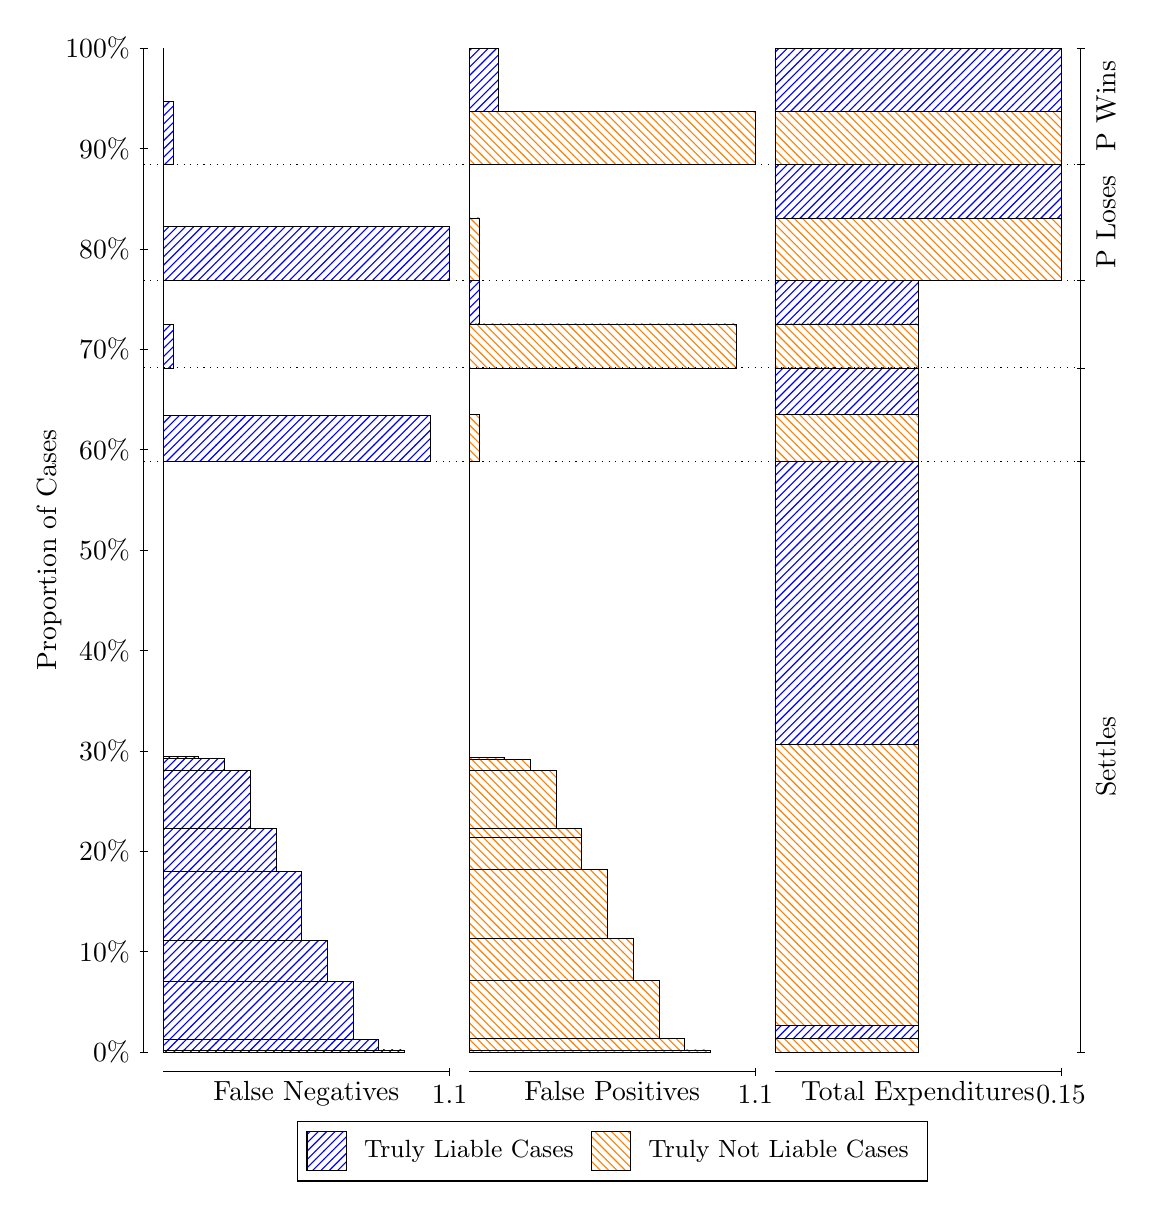
\begin{tikzpicture}
\draw[black, very thin] (1.5,1.75) -- (1.5,14.5);
\node[rotate=90, anchor=center] at (0.3, 8.125) {Proportion of Cases};
\draw[black, very thin] (1.45,1.75) -- (1.55,1.75);
\node[anchor=east] at (1.45, 1.75) {0\%};
\draw[black, very thin] (1.45,3.025) -- (1.55,3.025);
\node[anchor=east] at (1.45, 3.025) {10\%};
\draw[black, very thin] (1.45,4.3) -- (1.55,4.3);
\node[anchor=east] at (1.45, 4.3) {20\%};
\draw[black, very thin] (1.45,5.575) -- (1.55,5.575);
\node[anchor=east] at (1.45, 5.575) {30\%};
\draw[black, very thin] (1.45,6.85) -- (1.55,6.85);
\node[anchor=east] at (1.45, 6.85) {40\%};
\draw[black, very thin] (1.45,8.125) -- (1.55,8.125);
\node[anchor=east] at (1.45, 8.125) {50\%};
\draw[black, very thin] (1.45,9.4) -- (1.55,9.4);
\node[anchor=east] at (1.45, 9.4) {60\%};
\draw[black, very thin] (1.45,10.675) -- (1.55,10.675);
\node[anchor=east] at (1.45, 10.675) {70\%};
\draw[black, very thin] (1.45,11.95) -- (1.55,11.95);
\node[anchor=east] at (1.45, 11.95) {80\%};
\draw[black, very thin] (1.45,13.225) -- (1.55,13.225);
\node[anchor=east] at (1.45, 13.225) {90\%};
\draw[black, very thin] (1.45,14.5) -- (1.55,14.5);
\node[anchor=east] at (1.45, 14.5) {100\%};

\draw[black, very thin] (13.4,1.75) -- (13.4,14.5);
\draw[black, very thin] (13.35,1.75) -- (13.45,1.75);
\node[anchor=west] at (13.35, 1.75) {};
\draw[black, very thin] (13.35,9.2468) -- (13.45,9.2468);
\node[anchor=west] at (13.35, 9.2468) {};
\draw[black, very thin] (13.35,10.438) -- (13.45,10.438);
\node[anchor=west] at (13.35, 10.438) {};
\draw[black, very thin] (13.35,11.551) -- (13.45,11.551);
\node[anchor=west] at (13.35, 11.551) {};
\draw[black, very thin] (13.35,13.024) -- (13.45,13.024);
\node[anchor=west] at (13.35, 13.024) {};
\draw[black, very thin] (13.35,14.5) -- (13.45,14.5);
\node[anchor=west] at (13.35, 14.5) {};

\draw[black, very thin, pattern color=blue, pattern=north east lines] (1.75,1.75) rectangle (4.8118,1.7767);
\draw[black, very thin, pattern color=blue, pattern=north east lines] (1.75,1.7767) rectangle (4.4852,1.9138);
\draw[black, very thin, pattern color=blue, pattern=north east lines] (1.75,1.9138) rectangle (4.1586,2.6419);
\draw[black, very thin, pattern color=blue, pattern=north east lines] (1.75,2.6419) rectangle (3.832,3.1681);
\draw[black, very thin, pattern color=blue, pattern=north east lines] (1.75,3.1681) rectangle (3.5054,4.0472);
\draw[black, very thin, pattern color=blue, pattern=north east lines] (1.75,4.0472) rectangle (3.1788,4.585);
\draw[black, very thin, pattern color=blue, pattern=north east lines] (1.75,4.585) rectangle (2.8522,5.3284);
\draw[black, very thin, pattern color=blue, pattern=north east lines] (1.75,5.3284) rectangle (2.5257,5.4767);
\draw[black, very thin, pattern color=blue, pattern=north east lines] (1.75,5.4767) rectangle (2.1991,5.5035);
\draw[black, very thin, pattern color=orange, pattern=north west lines] (1.75,5.5035) rectangle (1.75,9.2468);
\draw[black, very thin, pattern color=blue, pattern=north east lines] (1.75,9.2468) rectangle (5.1384,9.8331);
\draw[black, very thin, pattern color=orange, pattern=north west lines] (1.75,9.8331) rectangle (1.75,10.438);
\draw[black, very thin, pattern color=blue, pattern=north east lines] (1.75,10.438) rectangle (1.8725,10.99);
\draw[black, very thin, pattern color=orange, pattern=north west lines] (1.75,10.99) rectangle (1.75,11.551);
\draw[black, very thin, pattern color=blue, pattern=north east lines] (1.75,11.551) rectangle (5.3833,12.231);
\draw[black, very thin, pattern color=orange, pattern=north west lines] (1.75,12.231) rectangle (1.75,13.024);
\draw[black, very thin, pattern color=blue, pattern=north east lines] (1.75,13.024) rectangle (1.8725,13.826);
\draw[black, very thin, pattern color=orange, pattern=north west lines] (1.75,13.826) rectangle (1.75,14.5);
\draw[black, very thin, pattern color=orange, pattern=north west lines] (5.6333,1.75) rectangle (8.6951,1.777);
\draw[black, very thin, pattern color=orange, pattern=north west lines] (5.6333,1.777) rectangle (8.3685,1.9225);
\draw[black, very thin, pattern color=orange, pattern=north west lines] (5.6333,1.9225) rectangle (8.0419,2.6616);
\draw[black, very thin, pattern color=orange, pattern=north west lines] (5.6333,2.6616) rectangle (7.7154,3.1918);
\draw[black, very thin, pattern color=orange, pattern=north west lines] (5.6333,3.1918) rectangle (7.3888,4.0642);
\draw[black, very thin, pattern color=orange, pattern=north west lines] (5.6333,4.0642) rectangle (7.0622,4.4783);
\draw[black, very thin, pattern color=orange, pattern=north west lines] (5.6333,4.4783) rectangle (7.0622,4.593);
\draw[black, very thin, pattern color=orange, pattern=north west lines] (5.6333,4.593) rectangle (6.7356,5.3219);
\draw[black, very thin, pattern color=orange, pattern=north west lines] (5.6333,5.3219) rectangle (6.409,5.4656);
\draw[black, very thin, pattern color=orange, pattern=north west lines] (5.6333,5.4656) rectangle (6.0824,5.4934);
\draw[black, very thin, pattern color=blue, pattern=north east lines] (5.6333,5.4934) rectangle (5.6333,9.2468);
\draw[black, very thin, pattern color=orange, pattern=north west lines] (5.6333,9.2468) rectangle (5.7558,9.8513);
\draw[black, very thin, pattern color=blue, pattern=north east lines] (5.6333,9.8513) rectangle (5.6333,10.438);
\draw[black, very thin, pattern color=orange, pattern=north west lines] (5.6333,10.438) rectangle (9.0217,10.998);
\draw[black, very thin, pattern color=blue, pattern=north east lines] (5.6333,10.998) rectangle (5.7558,11.551);
\draw[black, very thin, pattern color=orange, pattern=north west lines] (5.6333,11.551) rectangle (5.7558,12.344);
\draw[black, very thin, pattern color=blue, pattern=north east lines] (5.6333,12.344) rectangle (5.6333,13.024);
\draw[black, very thin, pattern color=orange, pattern=north west lines] (5.6333,13.024) rectangle (9.2667,13.698);
\draw[black, very thin, pattern color=blue, pattern=north east lines] (5.6333,13.698) rectangle (6.0007,14.5);
\draw[black, very thin, pattern color=orange, pattern=north west lines] (9.5167,1.75) rectangle (11.333,1.9215);
\draw[black, very thin, pattern color=blue, pattern=north east lines] (9.5167,1.9215) rectangle (11.333,2.0853);
\draw[black, very thin, pattern color=orange, pattern=north west lines] (9.5167,2.0853) rectangle (11.333,5.6572);
\draw[black, very thin, pattern color=blue, pattern=north east lines] (9.5167,5.6572) rectangle (11.333,9.2468);
\draw[black, very thin, pattern color=orange, pattern=north west lines] (9.5167,9.2468) rectangle (11.333,9.8513);
\draw[black, very thin, pattern color=blue, pattern=north east lines] (9.5167,9.8513) rectangle (11.333,10.438);
\draw[black, very thin, pattern color=orange, pattern=north west lines] (9.5167,10.438) rectangle (11.333,10.998);
\draw[black, very thin, pattern color=blue, pattern=north east lines] (9.5167,10.998) rectangle (11.333,11.551);
\draw[black, very thin, pattern color=orange, pattern=north west lines] (9.5167,11.551) rectangle (13.15,12.344);
\draw[black, very thin, pattern color=blue, pattern=north east lines] (9.5167,12.344) rectangle (13.15,13.024);
\draw[black, very thin, pattern color=orange, pattern=north west lines] (9.5167,13.024) rectangle (13.15,13.698);
\draw[black, very thin, pattern color=blue, pattern=north east lines] (9.5167,13.698) rectangle (13.15,14.5);
\draw[black, dotted] (1.5,9.2468) -- (13.4,9.2468);
\draw[black, dotted] (1.5,10.438) -- (13.4,10.438);
\draw[black, dotted] (1.5,11.551) -- (13.4,11.551);
\draw[black, dotted] (1.5,13.024) -- (13.4,13.024);
\draw[black, very thin] (1.75,1.5) -- (5.3833,1.5);
\node[anchor=north] at (3.5667, 1.5) {False Negatives};
\draw[black, very thin] (5.3833,1.45) -- (5.3833,1.55);
\node[anchor=north] at (5.3833, 1.45) {1.1};

\draw[black, very thin] (5.6333,1.5) -- (9.2667,1.5);
\node[anchor=north] at (7.45, 1.5) {False Positives};
\draw[black, very thin] (9.2667,1.45) -- (9.2667,1.55);
\node[anchor=north] at (9.2667, 1.45) {1.1};

\draw[black, very thin] (9.5167,1.5) -- (13.15,1.5);
\node[anchor=north] at (11.333, 1.5) {Total Expenditures};
\draw[black, very thin] (13.15,1.45) -- (13.15,1.55);
\node[anchor=north] at (13.15, 1.45) {0.15};

\node[black, centered, rotate=90] at (13.72, 5.4984) {Settles};


\node[black, centered, rotate=90] at (13.72, 12.287) {P Loses};
\node[black, centered, rotate=90] at (13.72, 13.762) {P Wins};

\draw (7.449999999999999,1.5) node[draw=none] (baseCoordinate) {};
\begin{scope}[align=center]
        \matrix[scale=0.5, draw=black, below=0.5cm of baseCoordinate, nodes={draw}, column sep=0.1cm]{
            \node[rectangle, draw, minimum width=0.5cm, minimum height=0.5cm, pattern=north east lines, pattern color=blue] {}; &
            \node[draw=none, font=\small] (B) {Truly Liable Cases}; &
            \node[rectangle, draw, minimum width=0.5cm, minimum height=0.5cm, pattern=north west lines, pattern color=orange] {}; &
            \node[draw=none, font=\small] (B) {Truly Not Liable Cases}; \\
            };
\end{scope}

\end{tikzpicture}
\end{document}